
% !TeX spellcheck = de_DE

\documentclass{article}

\usepackage[ngerman]{babel}
\usepackage{graphicx}
\usepackage{indentfirst}
\usepackage{hyperref}
\usepackage{geometry}
\usepackage{changepage}
\usepackage{booktabs}
\usepackage{float}
\usepackage{tabulary}
\usepackage{xcolor}
\usepackage{multirow}
\usepackage{caption}
\usepackage{subcaption}
\usepackage{lscape}
\usepackage{colortbl}
\usepackage{listings}
\usepackage[normalem]{ulem}
\usepackage{longtable}

\graphicspath{ {./images/} }
\setlength\parindent{0pt}

\hypersetup{
    colorlinks,
    linkcolor={cyan!50!black},
    citecolor={blue!50!black},
    urlcolor={blue!80!black}
}

\makeatletter
\newcommand{\sectionauthor}[1]{
	{\parindent 0em \large \scshape Autor: #1 \par \nobreak \vspace*{1em}}
	\@afterheading
}
\makeatother

\title{Bibliotheksanwendung - Feinspezifikation}
\date{\today\\v1.1}
\author{
	Ivan Charviakou\\
	León Liehr\\
	Mohamad Najjar\\
	Jonas Picker\\
	Sergei Pravdin
}

\begin{document}
\maketitle
\begin{figure}[H]
	\centering
	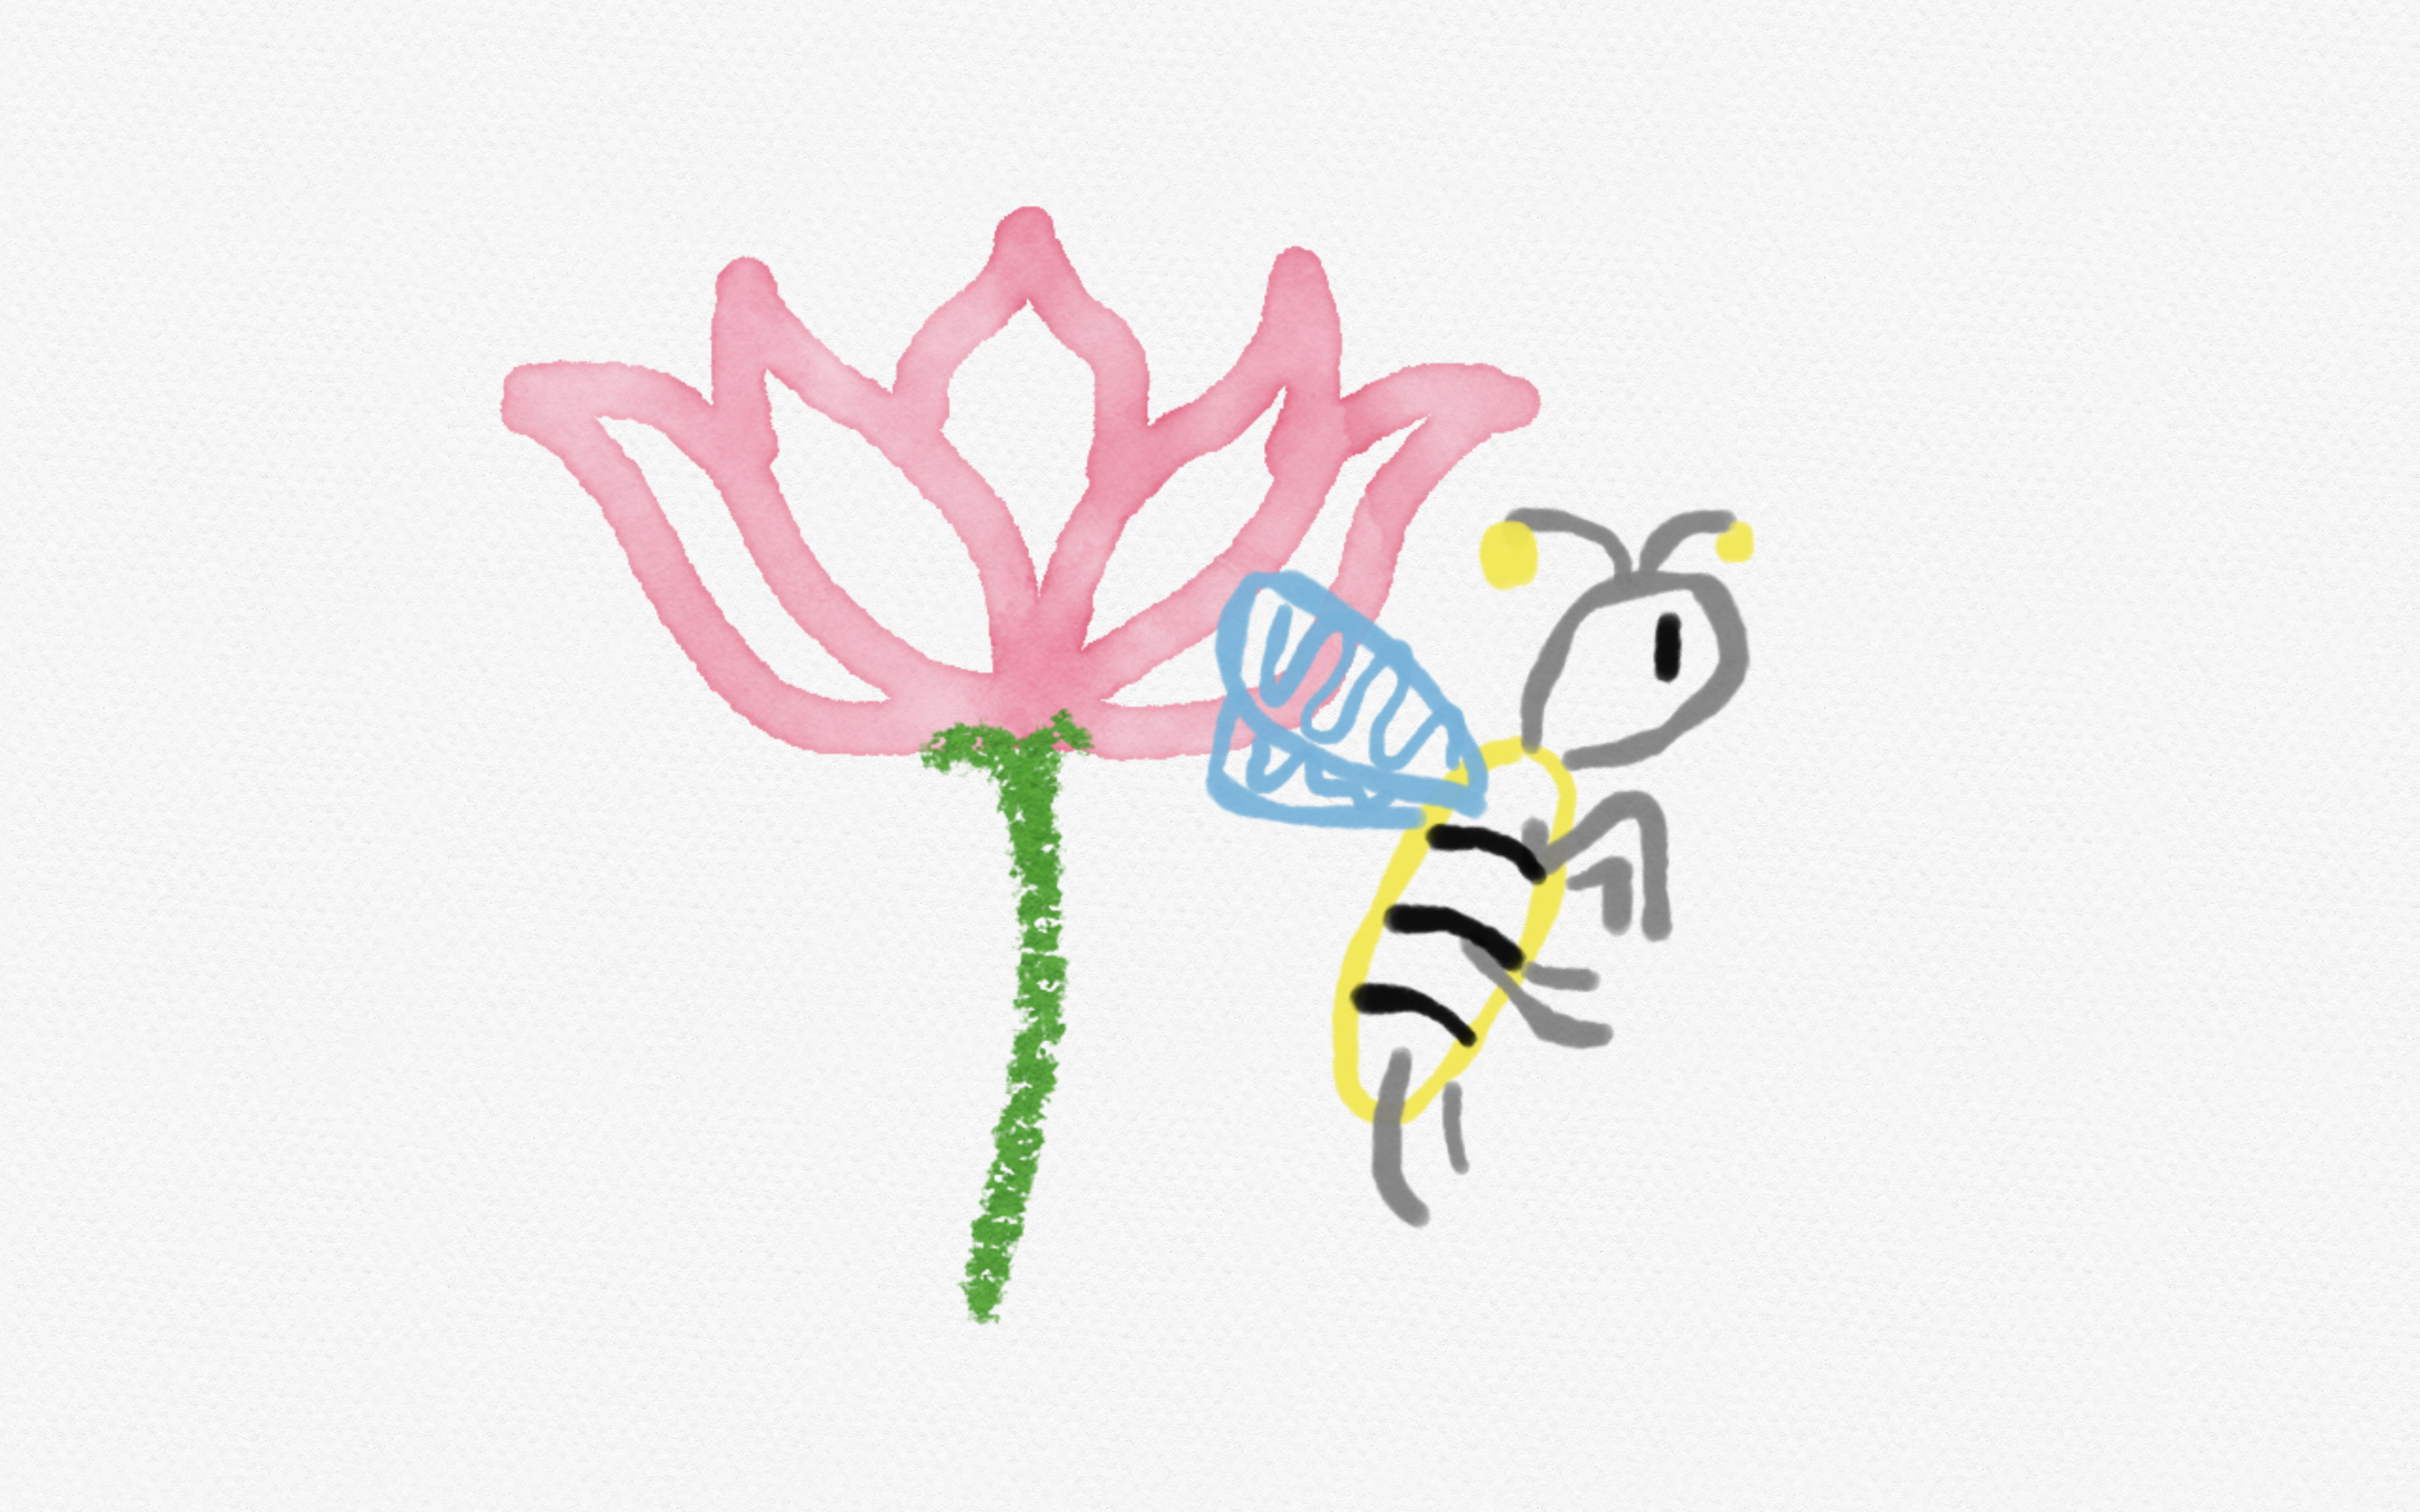
\includegraphics[width = 30em]{Logo}
\end{figure}
\newpage
\tableofcontents
\newpage

%----------------------------------------------------------------------Kapitel 0--------------------------------------------------------------------------------------------

\section{Einleitung}

In diesem Dokument ist der Implementierungsplan der Webanwendung \textbf{BiBi} dokumentiert. Dabei  erfolgt die Gliederung der Implementierung in Milestones, welche wiederum in Arbeitspakete aufgeteilt werden. Außerdem sind das \textbf{PERT-Diagramm},   die \textbf{Spezialgebiete}-Tabelle und die \textbf{Whitebox-Tests} zu sehen.

%----------------------------------------------------------------------Kapitel 1--------------------------------------------------------------------------------------------

\section{Meilensteine}
\sectionauthor{Jonas Picker}
Die Implementierungsphase wird drei Wochen dauern und in 3 gleiche Zeitabschnitte unterteilt, in denen wesentliche Funktionalitäten fertiggestellt werden sollen. Allgemein liegt der Schwerpunkt auf einer vertikale, testbare Realisierung einzelner Funktionen, jedoch müssen gewisse Kernmodule direkt im ersten Milestone abgearbeitet werden.
\subsection{Meilenstein 1}
\textbf{Fertigstellungsdatum:} 04.06.2021 \\
Im Fokus des ersten Meilensteins liegen Grundfunktionalitäten, nach seinem Erreichen soll das System auf normalem Wege gestartet und heruntergefahren werden können. Hierzu werden zunächst die Datenbankinitiallisierung und Anbindung, Fehlerbehandlung sowie System- und E-Mail-Konfiguration als horizontale Funktionspakete erstellt. Geplante vertikale Module des ersten Abschnitts beinhalten den Login und Registriervorgang für Benutzer sowie die Verwaltungsseite für Administratoren.
\subsection{Meilenstein 2}
\textbf{Fertigstellungsdatum:} 11.06.2021 \\
Der Hauptteil der essentiellen Systemfunktionen sollen im zweiten Abschnitt als vertikale Komponenten ausgearbeitet werden. Automatische Abläufe sowie die systemweite Sicherheit und Berechtigungsprüfung stehen an erster Stelle. Nach Erreichen des Meilensteins sollen Nutzer ihre Profildaten (außer E-Mail Reverifizierung) einsehen und verändern können, außerdem soll der Kategoriestöberer fertiggestellt werden. Die Mediumsansicht und Exemplarausleihe sowie Abarbeitungsfunktionalitäten für Mitarbeiter sind ebenfalls zu implementieren. Im gleichen Zug soll dann auch die Medienschemabearbeitung und das Erstellen neuer Medien ermöglicht werden.
\subsection{Meilenstein 3}
\textbf{Fertigstellungsdatum:} 18.06.2021 \\
In der letzten Implementierungsphase soll das System hauptsächlich um Randfunktionen ergänzt werden. Als letzter essentieller Block wird die Suchfunktionalität für Medien fertiggestellt. Mitarbeiter sollen eine Listenansicht mit abzuholenden Exemplaren und Leihfristverstößen angezeigt bekommen können. Für Nutzer soll ebenfalls eine Liste mit ausgeliehenen/abzuholenden Exemplaren einsehbar sein. Auch wird Nutzern die Passwort- und E-Mail-Zurücksetzung ermöglicht. Kleinere Komfortfunktionen wie z.B. das Anzeigen von Suchvorschlägen folgen zuletzt.

%----------------------------------------------------------------------Kapitel 2--------------------------------------------------------------------------------------------

\section{Arbeitspakete}

Die folgenden Tabellen dienen der Übersicht über die einzelnen Arbeitspakete, die zur Realisierung unseren System benötigt werden.
Sie geben unter Anderem die Klassen, Methoden, und Facelets an, die verschiedenen Arbeitspaketen innerhalb von Milestones zugeordnet sind. 
Dabei entsprechen die Tabellen den drei Milestones, die im Projekt vorgesehen sind.
Als Konvention wird vereinbart, dass wenn nur der Klassenname angegeben wird, die gesamte Klasse einschließlich aller Methoden zu implementieren ist. 
Analog steht ein Klassenattribut für die entsprechenden Getter- und Settermethoden.
Wird zusätzlich ein Methodenbezeichner angegeben, wird nur die Klassenmethode gemeint.

%----------------------------------------------------------------------Milestone 1--------------------------------------------------------------------------------------------

\subsection{Meilenstein 1}
Im Folgenden werden die Arbeitspakete, die zum Erreichen des ersten Milestones notwendig sind, aufgelistet und kurz beschrieben. Dabei steht BB für Backing Bean, C für Klasse, CC für Komponente, Co für Konverter, F für Facelet und M für Methode.

%\begin{center}

   % \begin{table}[H]

      %\begin{tabular} {| p{3cm} | p{6cm} |  p{3cm}  | %p{2.5cm}|  }
	%	\hline
	   %  \textbf{Arbeitspaket}& \textbf{Inhalt} & %\textbf{Entwickler} & \textbf{Dauer}\\
	     %\hline\hline
	     %Meta-implementation & Logger \newline %ConfigReader& Ivan Charviakou& ?\\ \hline
	    % Utilities I & ConnectionPool \newline %ApplicationDao\newline %ApplicationDto\newline CSSReader& Jonas %Picker& ?\\
	    % \hline

	     %Utilities II & EmailUtility \newline %HashingModule\newline & Ivan Charviakour& %?\\
	     %\hline

	   %  System I & SystemStartStop \newline %DataLayerInitializer\newline %Datenbankinitialisierung& Jonas Picker& ?\\
	     %\hline

	    %Faccelets I & Template \newline %Header\newline Footer\newline PaginatedList %und column &  León Liehr& ?\\
	    %\hline

	    %  Exception handling & Error  \newline %ErrorDto\newline Exceptions\newline Global %exception handler &  Sergei Pravdin& ?\\
	     %\hline

	     %  User definition & UserDto  \newline %UserSession\newline RoleConverter\newline %PasswordValidator\newline %ConfirmPasswordValidator \newline %EmailValidator \newline UserDao &  %Mohamad Najjar& ?\\
	     %\hline


	     %User authentication & UserDao  \newline %Registration\newline Login\newline %UserValidator &  Mohamad Najjar& ?\\
	     %\hline

	   %Application management global & SiteNotice  %\newline Contact\newline PrivacyPlocy &  %León Liehr & ?\\
	   %\hline

	    %Administrative functions& Administration  %\newline LogoValidator &  Sergei Pravdin& ?\\
	   %\hline

      %\end{tabular}
      %\caption{Tabelle des ersten Milestones}
    %\end{table}
%\end{center}

\newgeometry{top=1cm,bottom=1cm}
\begin{landscape}
	
	\begin{table}[H]
		\centering
		\begin{tabular}{llllll}
			\toprule
			\textbf{Arbeitspaket} &
			\textbf{ID} &
			\textbf{Inhalt} &
			\textbf{Abhängigkeiten} &
			\textbf{Entwickler} &
			\textbf{Dauer} \\
			\midrule
			Basis &
			11 &
			\begin{tabular}[c]{@{}l@{}}Logger (C)\\ ConfigReader (C)\\ \end{tabular} &
			11 &
			 Ivan Charviakou&
			5 \\
			Utilities I&
			10 &
			\begin{tabular}[c]{@{}l@{}}ConnectionPool  (C)\\ ApplicationDao (C)\\ ApplicationDto (C)\\ CSSReader (C)\\ \end{tabular} &
			11 &
			Jonas Picker &
			4  \\
			Utilities II&
			20 &
			\begin{tabular}[c]{@{}l@{}} EmailUtility (C)\\ TokenGenerator (C)\\ PasswordHashingModule (C)\end{tabular} &
			11 &
			Ivan Charviakou&
			4\\
			Systemstart&
			30 &
			\begin{tabular}[c]{@{}l@{}}SystemStartStop (C)\\DataLayerInitializer (C)\\ DatenbankInitialisierung (SQL)
		\end{tabular} &
			10 &
			Jonas Picker &
			4 \\
			Facelets &
			40 &
			\begin{tabular}[c]{@{}l@{}}Template (F) (BB)\\ PaginatedList (F)\\ \end{tabular} &
			10 &
			León Liehr &
			4 \\
			Fehlerbehandlung &
			41 &
		\begin{tabular}[c]{@{}l@{}}Fehlerseiten  (F) (BB)\\ ErrorDto (FC)\\ ExceptionHandler (C)\\ CustomExceptionHandler (C) \end{tabular}&
			40 &
			Sergei Pravdin &
			3 \\
			Nutzerdefinierung &
			52 &
			\begin{tabular}[c]{@{}l@{}}UserDto  (C) \\ UserSession (MB)\\ RoleConverter (Co)\\ PasswordValidator (C)\\ ConfirmPasswordValidator (C)\\ EmailValidator (C) \\ UserDao (M)\end{tabular}&
			30, 41 &
			Mohamad Najjar &
			6\\
			
			Nutzerathentifizierung &
			50 &
			\begin{tabular}[c]{@{}l@{}}UserDao  (M) \\ Registration (BB) (F)\\ Login (BB) (F)\\ UserValidator (C)\\ ConfirmPasswordValidator (C)\\ EmailValidator (C) \\ UserDao (M)\end{tabular}&
			52, 20 &
			Mohamad Najjar &
			4\\
			
			Globale Anwendungseinstellungen &
			61 &
			\begin{tabular}[c]{@{}l@{}}UserDao  (M) \\ Contact (BB) (F)\\ SiteNotice (BB) (F)\\ PrivacyPlocy (BB) (F)\\\end{tabular}&
			30, 41 &
			León Liehr &
			3\\
			
			Administrative Funktionalitäten &
			60 &
			\begin{tabular}[c]{@{}l@{}}Administration   (BB) (F) \\ LogoValidator (C)\\  \\\end{tabular}&
			30, 41 &
			Sergei Pravdin &
			4\\
			\bottomrule
		\end{tabular}
	 \caption{Tabelle des ersten Milestones}
	\end{table}
	
\end{landscape}
\restoregeometry

%----------------------------------------------------------------------Milestone 2--------------------------------------------------------------------------------------------

\subsection{Meilenstein 2}
\sectionauthor{Ivan Charviakou}

Im Folgenden werden die Arbeitspakete zum zweiten Meilenstein angegeben. Dabei wird die geschätzte Zeit in Stunden gemessen.

\begin{longtable}{|l|l|l|l|l|} 
\hline
\textbf{\uline{Arbeitspaket / Element}} & \textbf{\uline{ID / Inhalt}}             & \textbf{\uline{Abh.}}     & \textbf{\uline{Bearbeiter}} & \textbf{\uline{Zeit}}  \endfirsthead 
\hline
\textbf{\textit{Nutzerprofil}}          & \textbf{\textit{120}}                    & \textbf{\textit{50}}      & \textbf{\textit{Mohamad}}   & \textbf{\textit{3}}    \\ 
\hline
Facelet: Profilseite                    & profile.xhtml                            &                           &                             &                        \\ 
\hline
Backing-Bean: Profilseite               & Profile.init()                           &                           &                             &                        \\ 
\hline
                                        & Profile.user                             &                           &                             &                        \\ 
\hline
                                        & Profile.password                         &                           &                             &                        \\ 
\hline
                                        & Profile.confirmedPassword                &                           &                             &                        \\ 
\hline
                                        & Profile.delete()                         &                           &                             &                        \\ 
\hline
                                        & Profile.save()                           &                           &                             &                        \\ 
\hline
Session-Bean: Nutzer                    & UserSession.user                         &                           &                             &                        \\ 
\hline
DAO: Nutzer                             & UserDao.updateUser(…)                    &                           &                             &                        \\ 
\hline
                                        & UserDao.deleteUser(…)                    &                           &                             &                        \\ 
\hline
\textbf{\textit{Medienerstellung}}      & \textbf{\textit{80}}                     & \textbf{\textit{30, 41}}  & \textbf{\textit{Ivan}}      & \textbf{\textit{5}}    \\ 
\hline
Facelet: Medienerstellung               & medium-creator.xhtml                     &                           &                             &                        \\ 
\hline
Backing-Bean: Medienerstellung          & MediumCreator.init()                     &                           &                             &                        \\ 
\hline
                                        & MediumCreator.medium                     &                           &                             &                        \\ 
\hline
                                        & MediumCreator.copy                       &                           &                             &                        \\ 
\hline
                                        & MediumCreator.user                       &                           &                             &                        \\ 
\hline
                                        & MediumCreator.createMedium()             &                           &                             &                        \\ 
\hline
DTO: Medium                             & MediumDto.id                             &                           &                             &                        \\ 
\hline
                                        & MediumDto.category                       &                           &                             &                        \\ 
\hline
                                        & MediumDto.returnPeriod                   &                           &                             &                        \\ 
\hline
                                        & MediumDto.getAttribute(…)                &                           &                             &                        \\ 
\hline
                                        & MediumDto.setAttribute(…)                &                           &                             &                        \\ 
\hline
                                        & MediumDto.getCopy(…)                     &                           &                             &                        \\ 
\hline
                                        & MediumDto.setCopy(…)                     &                           &                             &                        \\ 
\hline
DAO: Medium                             & MediumDao.createMedium(...)              &                           &                             &                        \\ 
\hline
                                        & MediumDao.createCopy(...)                &                           &                             &                        \\ 
\hline
\textbf{\textit{Medienattribute}}       & \textbf{\textit{81}}                     & \textbf{\textit{30, 41}}  & \textbf{\textit{Jonas}}     & \textbf{\textit{5}}    \\ 
\hline
Facelet: Medienschema                   & medium-schema-editor.xhtml               &                           &                             &                        \\ 
\hline
Backing-Bean: Medienschema              & MediumSchemaEditor.init()                &                           &                             &                        \\ 
\hline
                                        & MediumSchemaEditor.addAttribute()        &                           &                             &                        \\ 
\hline
                                        & MediumSchemaEditor.deleteAttribute(...)  &                           &                             &                        \\ 
\hline
                                        & MediumSchemaEditor.save()                &                           &                             &                        \\ 
\hline
DTO: Attribut                           & AttributeDto.id                          &                           &                             &                        \\ 
\hline
                                        & AttributeDto.name                        &                           &                             &                        \\ 
\hline
                                        & AttributeDto.textValue                   &                           &                             &                        \\ 
\hline
                                        & AttributeDto.imageValue                  &                           &                             &                        \\ 
\hline
                                        & AttributeDto.urlValue                    &                           &                             &                        \\ 
\hline
                                        & AttributeDto.attributeModifiability      &                           &                             &                        \\ 
\hline
                                        & AttributeDto.type                        &                           &                             &                        \\ 
\hline
                                        & AttributeDto.attributeMultiplicity       &                           &                             &                        \\ 
\hline
                                        & AttributeDto.position                    &                           &                             &                        \\ 
\hline
DAO: Medium                             & MediumDao.updateGlobalAttributes(...)    &                           &                             &                        \\ 
\hline
                                        & MediumDao.readGlobalAttributes()         &                           &                             &                        \\ 
\hline
\textbf{\textit{Mediumansicht I}}       & \textbf{\textit{83}}                     & \textbf{\textit{30, 41}}  & \textbf{\textit{Sergei}}    & \textbf{\textit{5}}    \\ 
\hline
Facelet: Mediumansicht                  & medium.xhtml                             &                           &                             &                        \\ 
\hline
Backing-Bean: Mediumansicht             & Medium.init()                            &                           &                             &                        \\ 
\hline
                                        & Medium.saveAttributes()                  &                           &                             &                        \\ 
\hline
                                        & Medium.createCopy()                      &                           &                             &                        \\ 
\hline
                                        & Medium.deleteCopy()                      &                           &                             &                        \\ 
\hline
                                        & Medium.medium                            &                           &                             &                        \\ 
\hline
                                        & Medium.copy                              &                           &                             &                        \\ 
\hline
DTO: Exemplar                           & CopyDto.id                               &                           &                             &                        \\ 
\hline
                                        & CopyDto.location                         &                           &                             &                        \\ 
\hline
                                        & CopyDto.signature                        &                           &                             &                        \\ 
\hline
                                        & CopyDto.deadline                         &                           &                             &                        \\ 
\hline
                                        & CopyDto.copyStatus                       &                           &                             &                        \\ 
\hline
                                        & CopyDto.actor                            &                           &                             &                        \\ 
\hline
DAO: Medium                             & MediumDao.readCopy(...)                  &                           &                             &                        \\ 
\hline
                                        & MediumDao.updateMediumAttributes(…)      &                           &                             &                        \\ 
\hline
\textbf{\textit{Mediumansicht II}}      & \textbf{\textit{82}}                     & \textbf{\textit{83}}      & \textbf{\textit{Mohamad}}   & \textbf{\textit{5}}    \\ 
\hline
Backing-Bean: Mediumansicht             & Medium.getReturnPeriod()                 &                           &                             &                        \\ 
\hline
                                        & Medium.updateReturnPeriod()              &                           &                             &                        \\ 
\hline
                                        & Medium.saveCopy()                        &                           &                             &                        \\ 
\hline
                                        & Medium.lendCopy()                        &                           &                             &                        \\ 
\hline
                                        & Medium.returnCopy()                      &                           &                             &                        \\ 
\hline
                                        & Medium.pickUpCopy()                      &                           &                             &                        \\ 
\hline
                                        & Medium.cancelPickup()                    &                           &                             &                        \\ 
\hline
DAO: Medium                             & MediumDao.updateCopy(...)                &                           &                             &                        \\ 
\hline
                                        & MediumDao.deleteCopy(...)                &                           &                             &                        \\ 
\hline
\textbf{\textit{Kategoriesuche}}        & \textbf{\textit{110}}                    & \textbf{\textit{30, 41}}  & \textbf{\textit{Leon}}      & \textbf{\textit{4}}    \\ 
\hline
Facelet: Kategoriesuche                 & category-browser.xhtml                   &                           &                             &                        \\ 
\hline
Backing-Bean: Kategoriesuche            & CategoryBrowser.init()                   &                           &                             &                        \\ 
\hline
                                        & CategoryBrowser.categorySearch           &                           &                             &                        \\ 
\hline
                                        & CategoryBrowser.currentCategory          &                           &                             &                        \\ 
\hline
                                        & CategoryBrowser.deleteCategory()         &                           &                             &                        \\ 
\hline
                                        & CategoryBrowser.searchCategory()         &                           &                             &                        \\ 
\hline
                                        & CategoryBrowser.getItems()               &                           &                             &                        \\ 
\hline
DTO: Kategoriensuche                    & CategorySearchDto.searchTerm             &                           &                             &                        \\ 
\hline
DAO: Kategorie                          & CategoryDao.readCategory()               &                           &                             &                        \\ 
\hline
                                        & CategoryDao.readCategoriesByName()       &                           &                             &                        \\ 
\hline
\textbf{\textit{Kategorieerstellung}}   & \textbf{\textit{111}}                    & \textbf{\textit{30, 41}}  & \textbf{\textit{Leon}}      & \textbf{\textit{4}}    \\ 
\hline
Facelet: Kategorieerstellung            & category-creator.xhtml                   &                           &                             &                        \\ 
\hline
Backing-Bean: Kategorieerstellung       & CategoryCreator.init()                   &                           &                             &                        \\ 
\hline
                                        & CategoryCreator.category                 &                           &                             &                        \\ 
\hline
                                        & CategoryCreator.createCategory()         &                           &                             &                        \\ 
\hline
DTO: Kategorie                          & CategoryDto.id                           &                           &                             &                        \\ 
\hline
                                        & CategoryDto.name                         &                           &                             &                        \\ 
\hline
                                        & CategoryDto.description                  &                           &                             &                        \\ 
\hline
                                        & CategoryDto.parent                       &                           &                             &                        \\ 
\hline
DAO: Kategorie                          & CategoryDao.createCategory(…)            &                           &                             &                        \\ 
\hline
                                        & CategoryDao.updateCategory(…)            &                           &                             &                        \\ 
\hline
                                        & CategoryDao.deleteCategory(…)            &                           &                             &                        \\ 
\hline
\textbf{\textit{Medientransaktionen}}   & \textbf{\textit{90}}                     & \textbf{\textit{80, 120}} & \textbf{\textit{Sergei}}    & \textbf{\textit{4}}    \\ 
\hline
Facelet: Medienausleihe                 & lending.xhtml                            &                           &                             &                        \\ 
\hline
Backing-Bean: Medienausleihe            & Lending.init()                           &                           &                             &                        \\ 
\hline
                                        & Lending.user                             &                           &                             &                        \\ 
\hline
                                        & Lending.copies                           &                           &                             &                        \\ 
\hline
                                        & Lending.lendCopies()                     &                           &                             &                        \\ 
\hline
                                        & Lending.addSignatureInputField()         &                           &                             &                        \\ 
\hline
Facelet: Medienrückgabe                 & return-form.xhtml                        &                           &                             &                        \\ 
\hline
Backing-Bean: Medienrückgabe            & ReturnForm.init()                        &                           &                             &                        \\ 
\hline
                                        & ReturnForm.user                          &                           &                             &                        \\ 
\hline
                                        & ReturnForm.copies                        &                           &                             &                        \\ 
\hline
                                        & ReturnForm.returnCopies()                &                           &                             &                        \\ 
\hline
                                        & ReturnForm.addSignatureInputField()      &                           &                             &                        \\ 
\hline
DAO: Medium                             & MediumDao.lendCopy(...)                  &                           &                             &                        \\ 
\hline
                                        & MediumDao.returnCopy(...)                &                           &                             &                        \\ 
\hline
\textbf{\textit{Wartungsprozess}}       & \textbf{\textit{170}}                    & \textbf{\textit{10, 20}}  & \textbf{\textit{Jonas}}     & \textbf{\textit{3}}    \\ 
\hline
Klasse: Wartungsprozess                 & MaintenanceProcess.setTimeoutInterval(…) &                           &                             &                        \\ 
\hline
                                        & MaintenanceProcess.run()                 &                           &                             &                        \\ 
\hline
                                        & MaintenanceProcess.shutdown()            &                           &                             &                        \\ 
\hline
\textbf{\textit{Trespasslistener}}      & \textbf{\textit{161}}                    & \textbf{\textit{50}}      & \textbf{\textit{Ivan}}      & \textbf{\textit{3}}    \\ 
\hline
Klasse: Trespasslistener                & TrespassListener.beforePhase(…)          &                           &                             &                        \\ 
\hline
                                        & TrespassListener.afterPhase(…)           &                           &                             &                        \\ 
\hline
                                        & TrespassListener.getPhaseId()            &                           &                             &                        \\
\hline
\end{longtable}

%----------------------------------------------------------------------Milestone 3--------------------------------------------------------------------------------------------

\subsection{Meilenstein 3}
\sectionauthor{León Liehr}

Nachfolgend die Arbeitspakete des dritten Milestones. Dabei steht BB für Backing Bean, C für Klasse, CC für Komponente, Co für Konverter, F für Facelet und M für Methode.

\newgeometry{top=1cm,bottom=1cm}
\begin{landscape}

\begin{table}[H]
    \centering
    \begin{tabular}{llllll}
        \toprule
        \textbf{Arbeitspaket} &
        \textbf{ID} &
        \textbf{Inhalt} &
        \textbf{Abhängigkeiten} &
        \textbf{Entwickler} &
        \textbf{Dauer} \\
        \midrule
        Medium Search &
        130 &
        \begin{tabular}[c]{@{}l@{}}medium-search (F)\\ MediumSearch (BB)\\ searchMedium (M)\\ addNuancedSearchField (M)\\ MediumDao (C)\\ readMediaBySearchCriteria (M)MediumSearchDto (C)\\ AttributeOrCategoryConverter (Co)\\ AvailabilityStatusConverter (Co)\\ MediumPeviewPositionConverter (Co)\\ SearchOperatorConverter (Co)\end{tabular} &
        80, 81 &
        León Liehr &
        8 \\
        Password Reset \& Email Validation &
        150 &
        \begin{tabular}[c]{@{}l@{}}password-reset (F)\\ PasswordReset (BB)\\ resetPassword (M)\\ email-confirmation (F)\\ EmailConfirmation (BB)\\ confirmEmailAddress (M)\\ UserDao (C)\end{tabular} &
        120 &
        Ivan Charviakou &
        6 \\
        Copies of a User &
        100 &
        \begin{tabular}[c]{@{}l@{}}copies-ready-for-pickup (F)\\ CopiesReadyForPickup (BB)\\ borrowed-copies (F)\\ BorrowedCopies (BB)\\ MediumDao (C)\end{tabular} &
        80, 120 &
        Sergei Pravdin &
        5 \\
        Copies by User &
        91 &
        \begin{tabular}[c]{@{}l@{}}copies-ready-for-pickup-all-users (F)\\ CopiesReadyForPickupAllUsers (BB)\\ lending-period-violations (F)\\ LendingPeriodViolations (BB)\\ MediumDao (C)\end{tabular} &
        80, 120 &
        Jonas Picker &
        5 \\
        User Search &
        140 &
        \begin{tabular}[c]{@{}l@{}}user-search (F)\\ UserSearch (BB)\\ UserSearchDto (C)\\ UserDao (C)\end{tabular} &
        120 &
        Mohamad Najjar &
        6 \\
        Enhancements &
        160 &
        reactiveInputField (CC) &
        130, 140, 110 &
        León Liehr &
        3 \\
        \bottomrule
    \end{tabular}
    \caption{Tabelle des drtten Milestones}
\end{table}

\end{landscape}
\restoregeometry

%----------------------------------------------------------------------Kapitel 3--------------------------------------------------------------------------------------------

\section{PERT-Diagramm}
\sectionauthor{Ivan Charviakou}

Im Folgenden wird das PERT Diagramm zum Projekt dargestellt. Insbesondere bildet es die Abhängigkeiten zwischen den Paketen ab und zeigt das kritische Pfad im Projekt auf. Dabei werden die Zeitdauer in Stunden berechnet.

\begin{figure}[H]
	\centering
	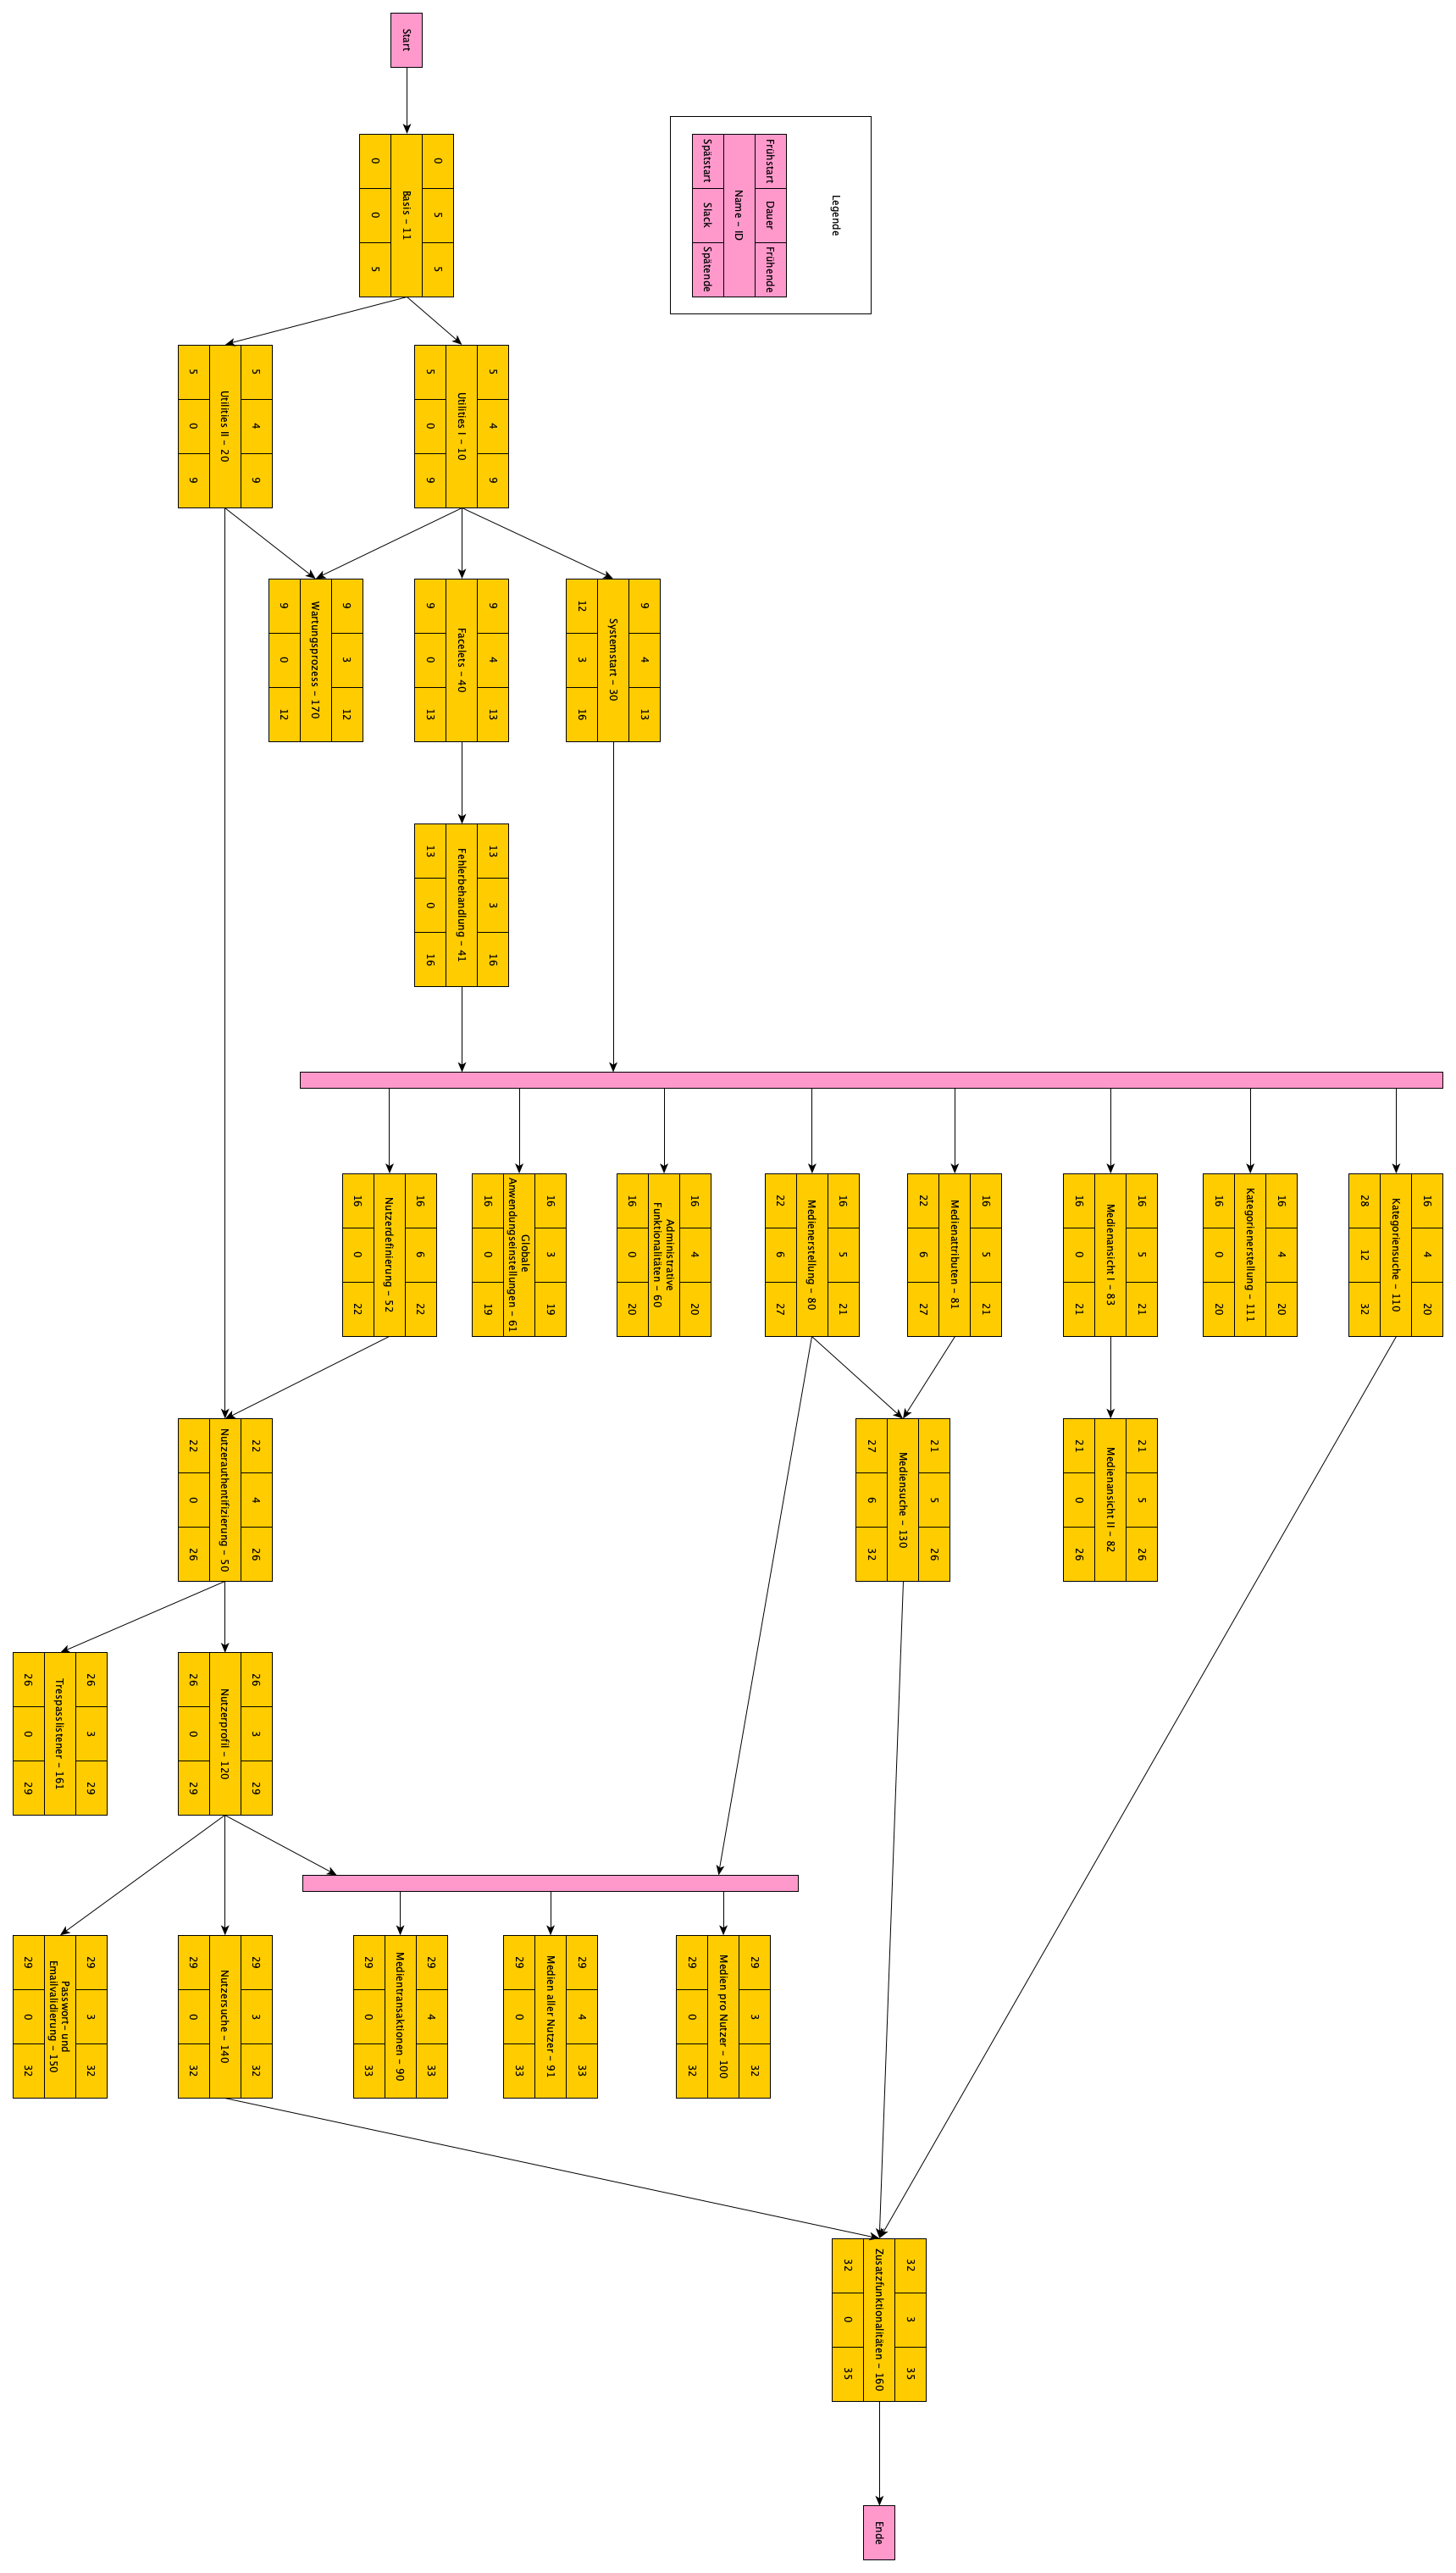
\includegraphics[width = 30em]{PERT}
\end{figure}

%----------------------------------------------------------------------Kapitel 4--------------------------------------------------------------------------------------------

\section{Spezialgebiete}
\sectionauthor{Jonas Picker}
Die Vielzahl der verwendeten Technologien erfordert eine Spezialisierung der einzelnen Teammitglieder. Die jeweiligen Spezialgebiete sind \hyperlink{speziell}{unten} aufgelistet.
\begin{table}[H]
\centering
\hypertarget{speziell}{}
\begin{tabular}{| p{6cm} | p{6cm} |}
	\hline
     	git & León Liehr \\
     	\hline
     	JSF Internationalisierung & León Liehr \\
     	\hline
    	JSF Templates & León Liehr \\
     	\hline
     	JSF Components & León Liehr \\
     	\hline
     	\hline
     	LaTeX & Ivan Charviakou \\
     	\hline
     	RegEx & Ivan Charviakou \\
     	\hline
     	Jakarta Mail & Ivan Charviakou \\
     	\hline
     	JSF Validators & Ivan Charviakou \\
     	\hline
     	\hline
     	JSF Converters & Mohamad Najjar \\
    	\hline
    	 RSA & Mohamad Najjar \\
    	\hline
    	 CSS/Bootstrap & Mohamad Najjar \\
     	\hline
     	Listenabstraktion & Mohamad Najjar \\
     	\hline
     	\hline
     	SQL & Jonas Picker \\
    	\hline
    	JSF File Upload & Jonas Picker \\
     	\hline
     	JSF/CDI Scopes & Jonas Picker \\
     	\hline
     	SSL/TLS & Jonas Picker \\
     	\hline
     	Systemkonfiguration & Jonas Picker \\
     	\hline
     	\hline
     	Selenium & Sergei Pravdin \\
     	\hline
     	Logging & Sergei Pravdin \\
     	\hline
     	JUnit & Sergei Pravdin \\
     	\hline
\end{tabular}
\end{table}

%----------------------------------------------------------------------Kapitel 5--------------------------------------------------------------------------------------------
\section{Whitebox-Tests}

\end{document}
